\section{Fast Nystr\"om Attention}
\label{sec:fna}

The emergence of massive tokens as attention sinks creates a highly structured and predictable pattern in the attention matrix, particularly in the middle-to-late layers of vision transformers. Once these tokens form, they dominate the attention distribution, creating a low-rank structure where most queries primarily attend to their immediate context and sink tokens(see Figure \ref{fig:attention_transition_layers}). This phenomenon suggests that the full attention matrix—while quadratic in size—can be efficiently approximated by preserving the critical interactions involving these key tokens while compressing less informative regions. 

\subsection{Formulation}
\label{sec:formulation}



% \subsubsection{Nystr\"om vs Nystr\"omFormer}
By leveraging token partitioning information, we can compress the attention matrix to achieve significant memory and speed improvements during inference. The primary objective is to construct a low-rank approximation of the attention matrix $\Ll{\ell}_hR_h^{(\ell)\top} \approx \Al{\ell}_h = \sf(\Ql{\ell}_h \mbf{K}^{(\ell)\top}_h / \sqrt{d})$ where $\Ll{\ell}_h, \Rl{\ell}_h \in \R^{(N + 1) \times s}$ for $s \ll N + 1$, which allows us to approximate the attention in $O(sND)$ time and space rather than $O(N^2D)$. The classical Nystr\"om extension suggests the approximation
\vspace{-4pt} \begin{align}
    \Al{\ell}_h
    \approx \Al{\ell}_{h, : \to S} (\Al{\ell}_{h, S \to S})^{-1} \Al{\ell}_{h, S \to :}
\end{align} where $S \subseteq [N]_0, \abs{S} = s$ represents the set of sampled tokens used for the quadrature approximation and $[N]_0$ represents the set of all integers from $0$ to $N$. However, we observe that exactly computing $\Al{\ell}_{h, : \to S}$ does not avoid quadratic complexity, as it would necessitate computation of all exponential row sums for the denominators of softmax. \cite{xiong2021nystromformer} resolves this issue by instead approximating with \vspace{-4pt} \begin{align}
    \resizebox{\columnwidth}{!}{$
        \Al{\ell}_h
        \approx \sf\pfrac{\Ql{\ell}_h k^{(\ell)\top}_h}{\sqrt{d}} \sf\pfrac{\ql{\ell}_h k^{(\ell)\top}_h}{\sqrt{d}}^{-1} \sf\pfrac{\ql{\ell}_h \mbf{K}^{(\ell)\top}_h}{\sqrt{d}}
    $}
\end{align}
% \begin{align}
% \resizebox{\columnwidth}{!}{$
%     \Al{\ell}_h
%     \approx \sf\pfrac{\Ql{\ell}_h \mbf{K}^{(\ell)\top}_{h, S}}{\sqrt{d'}} \sf\pfrac{\Ql{\ell}_{h, S} \mbf{K}^{(\ell)\top}_{h, S}}{\sqrt{d'}}^{-1} \sf\pfrac{\Ql{\ell}_{h, S} \mbf{K}^{(\ell)\top}_h}{\sqrt{d'}}
% $}
% \end{align}
where $\ql{\ell}_h, \kl{\ell}_h \in \R^{s \times d}$ are ``landmark features'' that approximate the set of tokens, opting to apply softmax on the intermediate matrices in spite of the discrepancy in softmax denominator.









\subsection{Methods}

% \subsubsection{How our work differs}
While our method of decomposition is drawn from \cite{xiong2021nystromformer}, our work differs in two key ways: 
\begin{enumerate}[label=\arabic*)]
    \item we opt for a universally-applicable training-free approach that aims to improve the efficiency of vision transformers without the need to modify the underlying model, and
    \vspace{-0.2cm}
    \item while \cite{xiong2021nystromformer} uses Segment-Means cluster centers as their landmark features, we instead choose to sample points directly from the set of tokens via Farthest Point Sampling (FPS) \cite{qi2017fps}, producing better results in comparison to Segment-Means and other training-free approaches, and bypassing the need to compute cluster centers at inference time.
\end{enumerate}


% \subsubsection{FPS configurations}
We identify CLS, massive tokens, and artifact tokens as three sets of tokens that we may wish to regard differently from the remainder of the tokens while sampling. Let $\fpsl{\ell}(S, k) = F$ denote the procedure in which we sample $k$ points from the block outputs $\cbn{\emb{\ell}{i}}_{i \in S}$ via farthest point sampling and return their indices so that $F \subseteq S$, $\abs{F} = k$. Then, given a ``guarantee'' set $G$ and an ``exclusion'' set $E$ where $G, E \subseteq [N]_0$ and $G \cap E = \emptyset$, we sample $s$ points from $\cbn{\emb{\ell}{CLS}, \emb{\ell}{0}, \ldots, \emb{\ell}{N}}$ by \begin{align}
    S = G \cup \fpsl{\ell}([N]_0 \setminus (G \cup E), s - \abs{G}).
\end{align} 
To simplify, we sample $s$ points with the guarantees that all points in $G$ are sampled, no point in $E$ is sampled, and the sample quota not covered by $\abs{G}$ is sampled from the remaining points via FPS. We can therefore regard each of the interest sets in three ways: to assign them to $G$ (``guarantee''), assign them to $E$ (``exclude''), or assign them to the FPS sampling pool $[N]_0 \setminus (G \cup E)$ (``ignore''), which results in a total of $3^3 = 27$ different configurations.

% \subsubsection{Our choice of FPS configuration}

In our Fast Nystr\"om Attention method, we guarantee the inclusion of the CLS token while using FPS to select the remaining tokens. This approach works effectively because massive and artifacts tokens are statistical outliers on the feature manifold, ensuring that FPS naturally represents the sink token population without over-saturating the subsample. In comparison to other sampling methods, we find that this performs nearly identical to guaranteeing the sampling of massive tokens, significantly better than guaranteeing the sampling of artifact tokens, and notably better than excluding either. We opt to ignore rather than guarantee massive tokens as it bypasses the need to explicitly extract them and instead relegate that task to the proficiencies of FPS. The details of these results are illustrated in Appendix \ref{sec:appendix_results_fna_sampling}.



\begin{table}[H]
    \centering
    \footnotesize
    \resizebox{\columnwidth}{!}{%
        \begin{tabular}{lcccc}
            \toprule
             & \multicolumn{2}{c}{Standard Attention} & \multicolumn{2}{c}{Fast Nystro\"m Attention \textbf{(ours)}} \\
            Sequence Length & Memory (MB) & Time (ms) & Memory (MB) & Time (ms) \\
            \midrule
            256 & 133 & 0.8 & 108 & 1.2 \\
            512 & 257 & 2.1 & 140 & 2.0 \\
            1,024 & 697 & 5.4 & 204 & 3.4 \\
            2,048 & 2,376 & 17.5 & 332 & 6.0 \\
            4,096 & 8,904 & 55.7 & 588 & 11.6 \\
            8,192 & 34,632 & 201.8 & 1,100 & 22.9 \\
            \bottomrule
        \end{tabular}%
    }
    \vspace{-0.5em}
    \caption{Memory consumption and running time results on various sequence lengths. We report the average memory consumption and running time for one input batch (batch size = 8) through a standard self-attention module (from scratch) and our Fast Nystr\"om Attention (sample size = 64). }
    \label{tab:nfa_speed_and_mem}
\end{table}




% \subsubsection{Complexity Analysis}

The main bottleneck of Fast Nystr\"om Attention lies in the FPS sampling step which is necessary to reduce the time complexity of the attention mechanism for each block from $O(N^2D)$ to $O(sND)$ and its space complexity to from $O(N^2 + ND)$ to $O(sN + ND)$. While the FPS subroutine itself requires $O(N^2D)$ time and $O(N^2)$ space to compute the pairwise distance matrix, we find that we can produce comparable results by sampling once after massive token formation and reusing those samples in the subsequent layers. This results in an overall reduction from $O(LN^2D)$ to $O(N^2D + sLND)$ in time, and while the peak memory consumption remains $O(N^2 + ND)$, it is reduced to $O(sN + ND)$ after Fast Nystr\"om Attention is applied. We compare the inference time and memory consumption of Fast Nystr\"om Attention with standard attention in Table \ref{tab:nfa_speed_and_mem}. 




\section{Experiments}

We implemented Fast Nystr\"om Attention as a PyTorch module that serves as a drop-in replacement for standard attention. We evaluated our approach on CLIP \cite{ilharco2021openclip} \cite{radford2021clip} and DINOv2 \cite{oquab2023dinov2} ViT L-14 models without any additional training or fine-tuning. Retrieval performance was assessed on COCO Captions \cite{chen2015coco} and Flickr30k \cite{young2014flickr} datasets using Recall@K metrics for bidirectional text-image retrieval. For vision-specific applications, we conducted zero-shot classification on ImageNet \cite{deng2009imagenet} and linear probing for semantic segmentation on VOC2012 \cite{pascal-voc-2012} and ADE20k \cite{zhou2017ade} datasets. All experiments were performed using a single NVIDIA RTX 4090 GPU.


\subsection{Pretrained Vision Backbones}


% \subsubsection{Say that FPS works}

Tables \ref{tab:fna_retrieval} and \ref{tab:fna_vision_only_results} summarize the results of applying Fast Nystr\"om Attention to CLIP and DINOv2. Our experiments show that Nystr\"om attention compression with FPS sampling delivers comparable results to standard attention on bidirectional retrieval, classification, and segmentation across multiple datasets. Notably, our one-time sampling strategy remains competitive with resampling at each layer and allows us to improve efficiency with only a minimal impact on performance metrics.

As seen in Table \ref{tab:fna_sampling_results}, Farthest Point Sampling runs only marginally slower than uniform random sampling while performing $~2\%$ better across all retrieval benchmarks, and outclasses other methods such as $k$-means and Spectral Clustering in both speed and performance. These results are supported by \cite{xiong2021nystromformer}, which shows that compression via Segment-Means requires retraining to achieve comparable results to standard attention. In addition, sampling methods that compute aggregate features (\textit{e.g.} Segment-Means) must be recomputed at every layer, unlike ``pure'' sampling methods.

There is an intuitive tradeoff between smaller sample sizes and model performance. Empirically, we find a sample size of 32 to 64 sufficient to approximate attention with competitive results to standard attention with no additional training (Appendix \ref{sec:appendix_results_fna_sampling}). Results of applying Fast Nystr\"om Attention to vision backbones of CLIP and DINOv2 are shown in Tables \ref{tab:fna_retrieval} and \ref{tab:fna_vision_only_results}. 


\begin{table}[t]
    \centering
    \footnotesize
    % Subtable (a): Image Retrieval
    \begin{subtable}[t]{\columnwidth}
        \centering
        \resizebox{\columnwidth}{!}{%
            \begin{tabular}{lcccccc}
                \toprule
                 & \multicolumn{3}{c}{COCO} & \multicolumn{3}{c}{Flickr30k} \\
                Model & R@1 & R@5 & R@10 & R@1 & R@5 & R@10 \\
                \midrule
                CLIP & 35.33 & 59.97 & 70.15 & 65.20 & 87.24 & 92.00  \\
                CLIP+FNA+no resample & 35.42 & 60.18 & 70.27 & 65.17 & 87.22 & 91.95 \\
                CLIP+FNA+resample & 35.58 & 60.43 & 70.51 & 65.27 & 87.25 & 91.98 \\
                \bottomrule
            \end{tabular}%
        }
        \caption{Image retrieval}
        \label{tab:fna_image_retrieval_sub}
    \end{subtable}
    
    \vspace{1em}
    
    % Subtable (b): Text Retrieval
    \begin{subtable}[t]{\columnwidth}
        \centering
        \resizebox{\columnwidth}{!}{%
            \begin{tabular}{lcccccc}
                \toprule
                 & \multicolumn{3}{c}{COCO} & \multicolumn{3}{c}{Flickr30k} \\
                Model & R@1 & R@5 & R@10 & R@1 & R@5 & R@10 \\
                \midrule
                CLIP & 56.06 & 79.48 & 86.84 & 85.10 & 97.30 & 99.00 \\
                CLIP+FNA+no resample & 55.39 & 78.72 & 86.49 & 85.06 & 97.16 & 98.78 \\
                CLIP+FNA+resample & 55.60 & 79.04 & 86.65 & 85.13 & 97.29 & 98.99 \\
                \bottomrule
            \end{tabular}%
        }
        \caption{Text retrieval}
        \label{tab:fna_text_retrieval_sub}
    \end{subtable}
    \vspace{-1em}
    \caption{Zero-shot retrieval results for CLIP ViT L-14 on COCO \cite{chen2015coco} and Flickr30k \cite{young2014flickr}. Our Fast Nystr\"om Approximation (FNA) with a sample size of 64 achieves competitive results with standard CLIP with no finetuning necessary.}
    \label{tab:fna_retrieval}
\end{table}

\begin{table}[t]
    \centering
    \footnotesize
    \resizebox{\columnwidth}{!}{%
        \begin{tabular}{lcccccc}
            \toprule
             & \multicolumn{2}{c}{ImageNet} & \multicolumn{2}{c}{VOC2012} & \multicolumn{2}{c}{ADE20k} \\
            Model & Top1 & Top5 & aACC & mIoU & aACC & mIoU \\
            \midrule
            CLIP & 75.96 & 94.82 & 90.33 & 66.60 & 69.55 & 34.84 \\
            CLIP+FNA+no resample & 75.74 & 94.49 & 90.19 & 66.53 & 69.18 & 34.64 \\
            CLIP+FNA+resample & 75.81 & 94.82 & 90.24 & 66.57 & 69.25 & 34.67 \\
            \midrule
            DINOv2 & 78.62 & 92.91 & 94.12 & 77.54 & 78.65 & 44.48 \\
            DinoV2+FNA+no resample & 78.57 & 92.89 & 93.91 & 77.35 & 78.46 & 44.40 \\
            DinoV2+FNA+resample & 78.60 & 92.92 & 93.98 & 77.41 & 78.49 & 44.42 \\
            \bottomrule
        \end{tabular}%
    }
    \vspace{-0.5em}
    \caption{Classification and segmentation benchmarks for pretrained CLIP and DINOv2 ViT L-14 show that Our Fast Nystr\"om Approximation (FNA) with a sample size of 64 achieves competitive results on dense vision tasks with no finetuning. ImageNet \cite{deng2009imagenet} classification evaluation is performed in the zero-shot setting. Segmentation on VOC2012 \cite{pascal-voc-2012} and ADE20k \cite{zhou2017ade} is performed via fitting linear probes to output of the final layers.}
    \label{tab:fna_vision_only_results}
\end{table}









% \subsubsection{FPS works better than other sampling methods}


\begin{table}[t]
    \centering
    \footnotesize
    \resizebox{\columnwidth}{!}{%
        \begin{tabular}{lccccc}
            \toprule
             &  & \multicolumn{2}{c}{Text-to-Image} & \multicolumn{2}{c}{Image-to-Text} \\
            Model & Time (s) & R@1 & R@5 & R@1 & R@5 \\
            \midrule
            CLIP+FNA (Multiclass SC)    & 1572.12           & 34.22             & 59.09             & 54.04             & 77.90 \\
            CLIP+FNA (SC)               & 1563.95           & 35.36             & 59.99             & 55.68             & 79.06 \\
            CLIP+FNA (K-Means)          & 875.05            & 35.33             & 60.11             & 55.28             & \textbf{79.40} \\
            CLIP+FNA (Segment-Means) \cite{xiong2021nystromformer}    & 74.27             & 32.96             & 57.80             & 49.32             & 74.18 \\
            CLIP+FNA (Uniform)          & \textbf{56.63}    & 33.77             & 58.66             & 53.90             & 77.96 \\
            \midrule
            CLIP+FNA (FPS)              & 61.25             & \textbf{35.91}    & \textbf{60.43}    & \textbf{56.52}    & 79.32 \\
            \bottomrule
        \end{tabular}%
    }
    \vspace{-0.5em}
    \caption{Zero-shot retrieval time and performance results on COCO for CLIP ViT L-14 and its Fast Nyström Approximation (FNA) with different sampling strategies.}
    \label{tab:fna_sampling_results}
\end{table}




% \subsubsection{Performance vs. sample size}

% \begin{figure}[t]
%     \centering
%     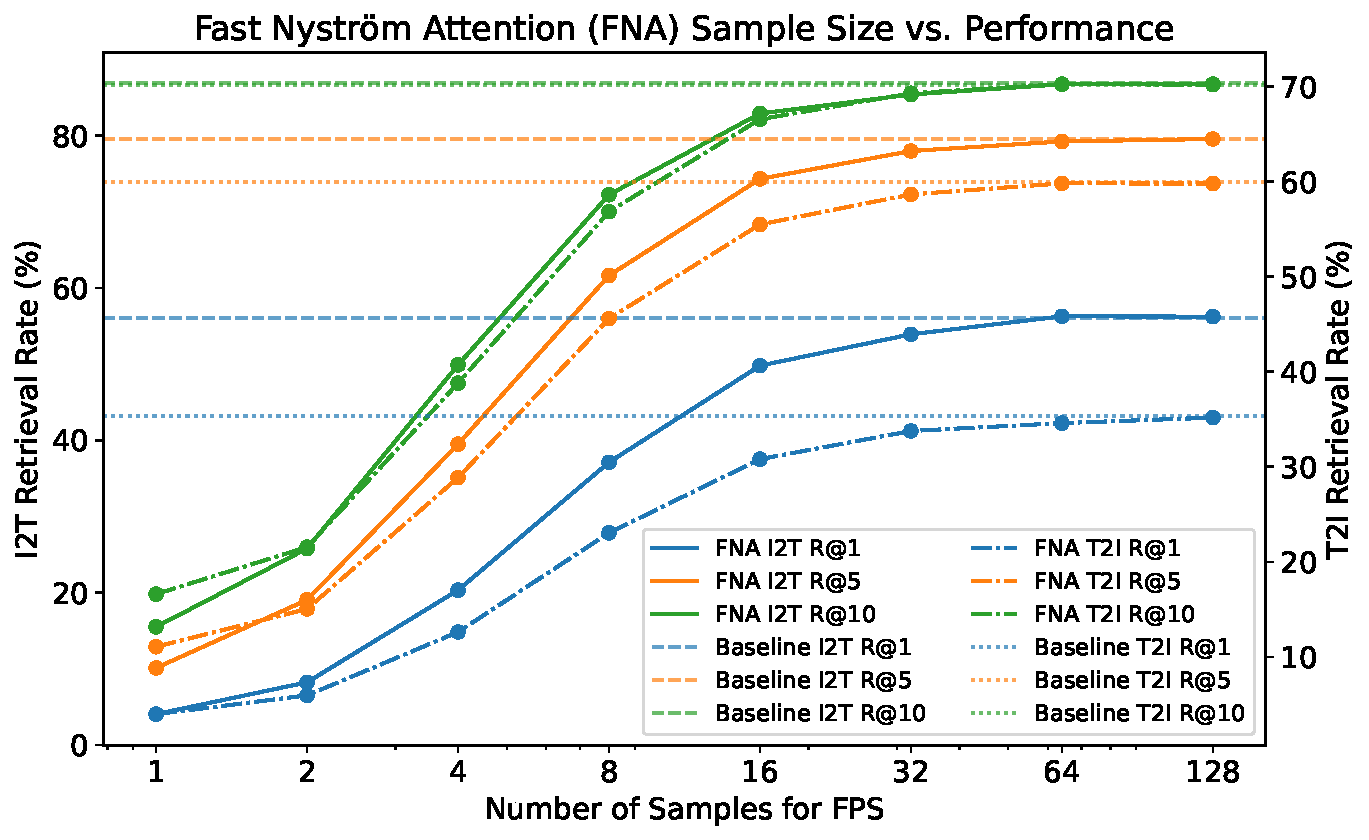
\includegraphics[width=1\linewidth]{figs/fna_sample_size_vs_performance.pdf}
%     \caption{Furthest point sampling (FPS) sample size vs. performance for COCO retrieval with CLIP ViT L-14 at 224x224px input resolution. (MOVE TO APPENDIX)}
%     \label{fig:fna_sample_size}
% \end{figure}



\subsection{Comparison with Existing Efficient Attention}
We benchmark Fast Nystr\"om Attention against existing efficient attention methods in Figure \ref{fig:attention_timing}, where it demonstrates highly competitive scaling. Compared to other linear scaling approximations \cite{choromanski2020performer} \cite{wang2020linformer}, our method is faster and training-free, allowing it to be applied as a drop-in replacement. While optimized exact attention like FlashAttention \cite{dao2024flashattention2} is popular, it remains fundamentally quadratic in time complexity. Results after finetuning are shown in Appendix \ref{sec:appendix_results_linear}.


\begin{figure}[t]
    \centering
    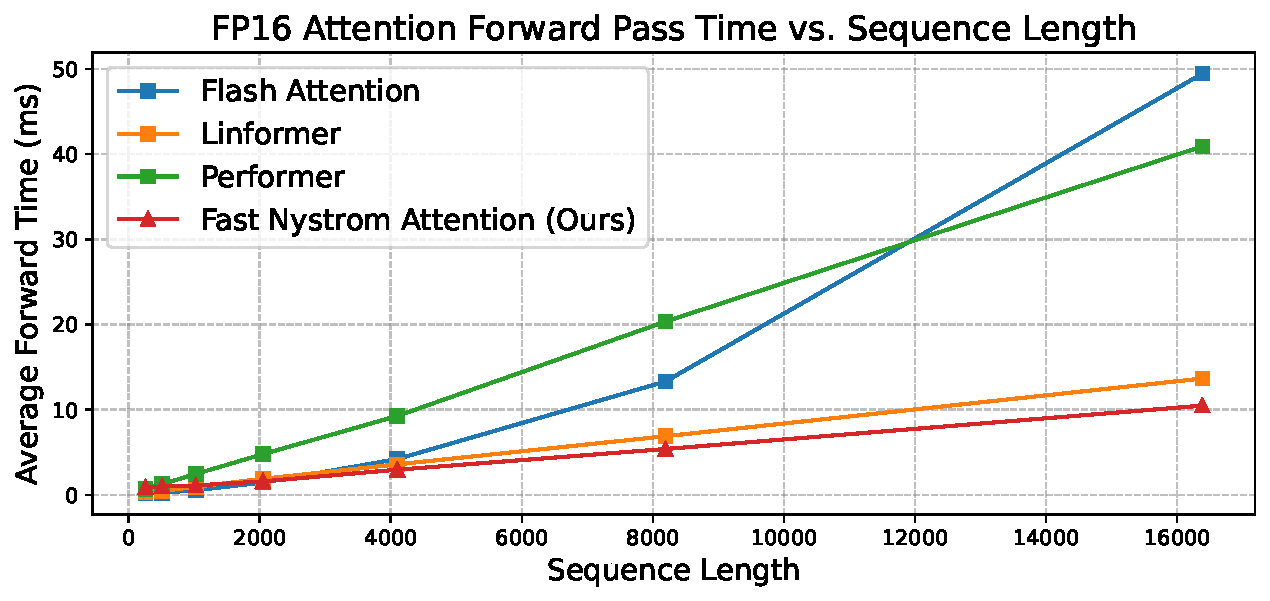
\includegraphics[width=1\linewidth]{figs/fp16_attention_timing_plot.pdf}
    \vspace{-2em}
    \caption{Fast Nyström Attention outperforms existing linear attention methods \cite{choromanski2020performer} \cite{wang2020linformer} in inference speed and offers superior scaling to FlashAttention \cite{dao2024flashattention2}.}
    \label{fig:attention_timing}
\end{figure}


\subsection{Vision Language Models}
We extend Fast Nyström Attention to LLaVA-NEXT-7B \cite{liu2023llava}, a vision-language model (VLM) composed of a pretrained image encoder and a large language model (LLM). In its standard operation, LLaVA processes an image into a large sequence of approximately 2500 tokens. These visual tokens are then incorporated into the LLM's causal attention mechanism to guide text generation, creating a significant computational load. While our reduction technique can be applied directly to LLaVA's vision encoder (as done for CLIP and DINOv2), reducing the tokens after they are projected into the LLM's text-embedding space proves more effective. Specifically, Nyström approximation is applied to the embedded image tokens within the LLaMA model, caching a compressed set of keys and values. This compact representation is then used for all subsequent causal attention steps, accelerating the generation of the text response. We evaluate on COCO VQA \cite{AgrawalCOCOVQA}, and report BERTScore \cite{Zhang2020BERTScore} between generated responses and ground-truth answers. As shown in Figure \ref{fig:llava_bert_scores}, Fast Nyström Attention boosts token throughput by 10\% while maintaining baseline performance. Qualitative examples are available in Appendix \ref{sec:appendix_results_llava}.


\begin{figure}[t]
    \centering
    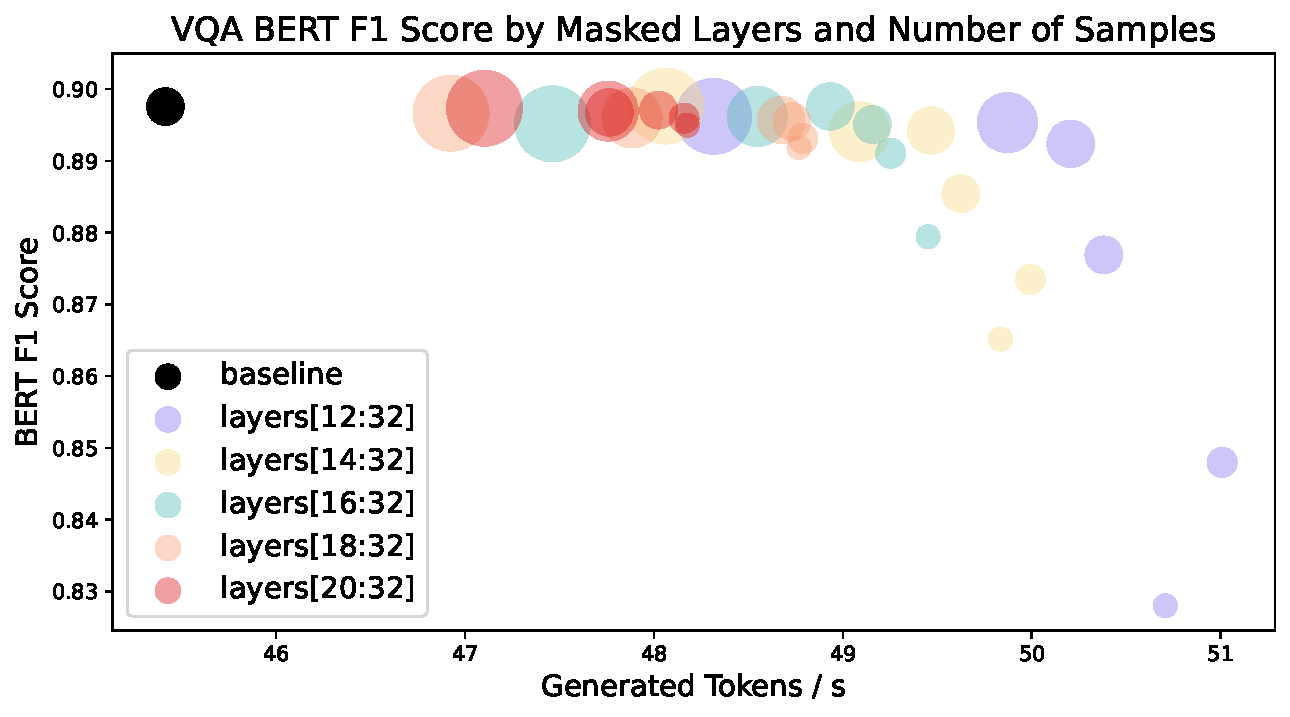
\includegraphics[width=1\linewidth]{figs/llava_vqa_bert_f1.pdf}
    \vspace{-2em}
    \caption{BERTScore \cite{Zhang2020BERTScore} and generation speed on COCO VQA \cite{AgrawalCOCOVQA} for different configurations of Fast Nystr\"om Attention (FNA) applied to LLaVA-NeXT-7B \cite{liu2023llava}. Each color represents a LLaVA model with FNA applied on the causal attention to image tokens at the specified span of layers. Spot size represent FNA sample sizes ranging from 16 to 512 tokens out of $\sim2500$ image tokens. 
    }
    \label{fig:llava_bert_scores}
\end{figure}

